\section{Configurazione}
	\subsection{Attività}
		\subsubsection{Gestione modifiche}
		Per effettuare una modifica ad un qualsiasi documento è necessario inoltrare una richiesta formale di modifica al \insrole{Responsabile di Progetto}, il quale si preoccuperà di avviare le procedure necessarie alla gestione di tale modifica.
		\subsubsection{Controllo di versione}
		Il controllo sul versionamento dei documenti e, nelle successive fasi del progetto, dei codice sorgente avviene attraverso lo strumento fornito dalla piattaforma GitHub.
		Ogni volta che viene eseguita una modifica sostaziale deve essere assegnato un nuovo numero di versione.\\ Il numero di versione è indicato attraverso il caarattere 'v' seguito da due numeri separati da un '.', dove il primo numero indica la versione approvata e il secondo il numero della verifica apportata.\\ Questo vale sia per i documenti che per i file contenenti codice sorgente.\\
		Per quanto riguarda il versionamento della documentazione si rimanda alla sezione Documentazione del presente documento.
	\subsection{Norme}
		\subsubsection{Struttura di una richiesta di modifica}
			Ogni richiesta di modifica è costituita dai seguenti campi:
			\begin{enumerate}
				\item Autore: contiene nome e cognome di colui che richiede la modifica;
				\item Documento: contiene il nome del documento di cui si richiede la modifica;
				\item Motivo: contiene la spiegazione chiara e concisa delle motivazioni per cui si sta richiedendo una modifica;
				\item Urgenza: può assumere uno dei seguenti valori:
					\begin{enumerate}
						\item Alta: si tratta di una modifica importante, con forti conseguenze nell'organizzazione e nello svolgimento delle attività future del progetto;
						\item Media: si tratta di una modifica importante, ma che non comporta grandi modifiche alle attività del progetto;
						\item Bassa: si tratta di una modifica di importanza secondaria, che può essere rimandata ad un secondo momento senza che ciò influisca in alcun modo sullo svoglimento delle attività.
					\end{enumerate}
			\end{enumerate}
			In seguito alla decisione del \insrole{Responsabile} di approvare o meno la richiesta, va aggiunto il campo:
			\begin{itemize}
				\item [5.] Decisione del \insrole{Responsabile di Progetto}: contiene uno dei seguenti valori:
					\begin{itemize}
						\item [-] Approvata
						\item [-] Respinta
					\end{itemize}
			\end{itemize}
	
		\subsubsection{Struttura del repository}
				I file all’interno del repository sono organizzati secondo la seguente struttura:
				\begin{itemize}
					\item /Documents
					\begin{itemize}
						\item Commons
						\item NormeDiProgetto
						\item StudioDiFattibilità
						\item AnalisiDeiRequisiti
						\item PianoDiProgetto
						\item PianoDiQualifica
						\item Verbali
						\item Glossario
					\end{itemize}
					\item /Source
				\end{itemize}
				La struttura di /Source viene definita prima della progettazione architetturale.

		\subsubsection{Nomi dei file}
				I nomi dei file all’interno del repository sono soggetti alle seguenti norme:
				\begin{itemize}
					\item devono contenere solamente lettere, numeri, il carattere underscore U+005F, il segno meno U+2212 e il punto U+002E;
					\item devono avere una lunghezza minima di 3 caratteri;
					\item devono contenere le informazioni sufficienti per distinguere il file in modo non ambiguo;
					\item le informazioni devono essere riportate dal generale al particolare;
					\item le date devono essere specificate nel formato YYYYMMDD.
				\end{itemize}
				Si consiglia inoltre:
				\begin{itemize}
					\item di utilizzare il meno possibile i caratteri underscore e segno meno, utilizzando al loro posto la notazione camel case;
					\item di utilizzare nomi con una lunghezza compresa tra i 5 e i 25 caratteri;
					\item di specificare sempre l’estensione quando possibile.
				\end{itemize}
			\subsubsection{Commit}
				L'esecuzione di un comando di commit implica il rispetto delle seguenti norme:
				\begin{itemize}
					\item quando si effettua un commit è necessario specificare nel messaggio una descrizione sintetica e non ambigua delle modifiche apportate;
					\item le modifiche apportate con un commit devono essere complete e testate con successo;
					\item le modifiche apportate con un commit devono essere logicamente correlate tra di loro.
				\end{itemize}
		\subsubsection{Codifica dei file}
			Tutti i file contenenti codice o documentazione dovranno utilizzare la codifica UTF-8 senza BOM.\\
			Il terminatore di linea è il carattere Line Feed, rappresentato dal carattere Unicode U+000A.
	
	\subsection{Procedure}
		\subsubsection{Richiesta di modifica}
		Ogni richiesta di modifica va inoltrata in modo formale al \insrole{Responsabile di Progetto}, affichè venga sottoposta ad un rigoroso processo di analisi. Dopodichè il \insrole{Responsabile di Progetto} decide se approvarla o meno. Nel primo caso assegna la realizzazione della modifica ad un membro del gruppo. Una volta effettuata la modifica, questa deve essere sottoposta a verifica. Tutto ciò deve avvenire mantenendo traccia dello stato precedente.
		
		\subsubsection{Aggiornamento del repository}
				Per aggiornare il repository è prevista una procedura ben definita, riportata nel seguente diagramma:
				\begin{figure}[H]
					\centering
					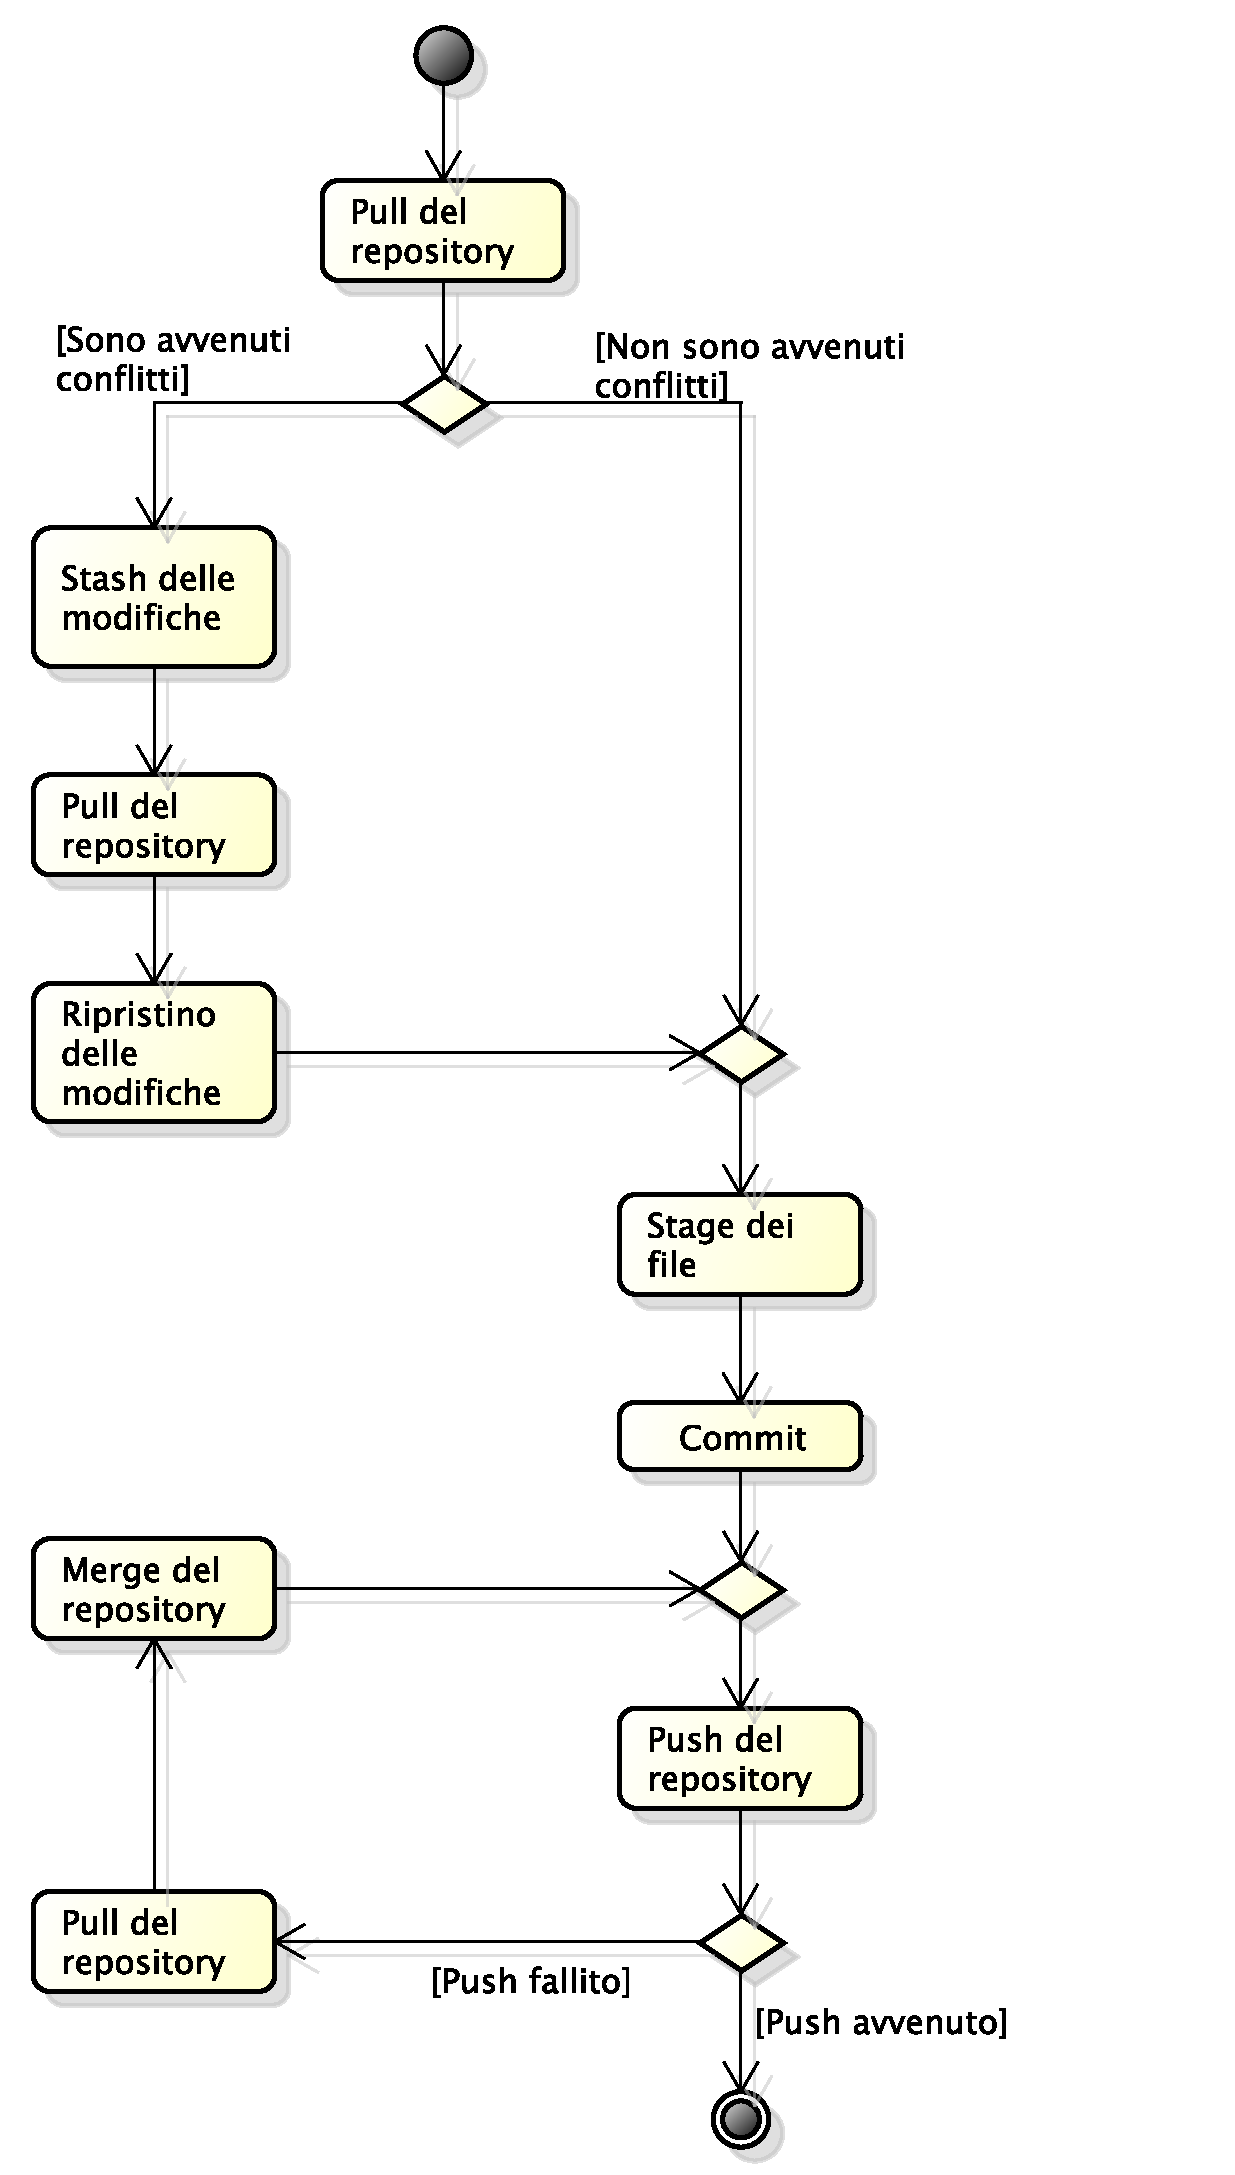
\includegraphics[width=0.6\textwidth]{NormeDiProgetto/Pics/Commit}
					\caption{Procedura di aggiornamento del repository}
				\end{figure}
		
	\subsection{Strumenti}
		Per agevolare lo svolgimento del progetto da parte di tutti i membri del team di sviluppo è stata predisposta una macchina virtuale contenente tutti gli strumenti software necessari, individuati fino al momento della stesura dell'ultima versione attuale del presente documento.
		\subsubsection{Repository}\label{sec:SceltaRepository}
			Per la gestione del repository si è scelto di utilizzare il sistema di versionamento distribuito Git. Questa scelta è stata presa in considerazione del fatto che questa piattaforma permette, oltre al servizio di \textit{repository}, il controllo di versione e la gestione di anomalie. \\
			GitHub è anche stato suggerito dal proponente del capitolato, in quanto permette un'interazione agevolata con Heroku, altro strumento consigliato per lo svolgimento del progetto. 
				\paragraph{Visibilità del repository}
				Per la condivisione e il versionamento dei configuration item è stato creato un repository privato su GitHub, raggiungibile all’indirizzo \insuri{https://github.com/marcorubin/kaizen-team}. L’accesso è consentito solamente agli utenti approvati dal \insrole{Project Manager}.
				